\documentclass[12pt, letterpaper]{article}
\usepackage[utf8]{inputenc}
\usepackage{graphicx}
\usepackage{apacite}
\usepackage{amsmath}


\title{{\huge Activación}}
\date{Febrero, 2018}
\author{Stéphane Lejars \& José Manuel García Niño}

\begin{document}

\maketitle
	
	Todo organismo debe adaptarse a su entorno, es decir, encontrar reglas que predicen regularmente una relación entre la variabilidad del entorno (propiedades estadísticas del entorno), y la variabilidad de su propia conducta (recordemos la restricción lineal del comportamiento).

	Para establecer estas reglas el organismo debe ejecutar diferentes conductas filogenéticas (conductas predeterminadas y específicas de una especie) que le permiten explorar el ambiente en el que se encuentra, por ejemplo, una rata olfatea y rasca en lugares donde podría encontrar comida, y evita aquellos lugares que ya han sido explorados anteriormente. 

	Eventualmente, el organismo, ya sea por su propia acción o por hazar, encontrará algo de valor (comida, o una pareja); la ocurrencia de este estímulo provocará un incremento de actividad, un esfuerzo adicional por parte del organismo para obtener más reforzamiento. Como ejemplo, imagina una situación familiar, cuando aventamos comida a un perro, este, al consumir el alimento, olfateará, por cierto periodo, los alrededores de donde encontró el alimento. Este incremento de actividad es lo que se conoce como \textbf{\textit{arousal}}, o, activación.

	La excitación es un incremento de actividad, y se supone, un incremento atencional hacia los estímulos externos, una interpretación plausible es que el organismo está buscando una causa posible a la aparición del estímulo (asignación de crédito),esto permite que se establezca una regla apropiada entre la conducta y el reforzador. La selección de la regla depende de conductas pre-establecidas apropiadas para la ocurrencia del reforzador, y de eventos temporales. \cite{staddon}
	
	\cite{killeen}, midieron activación en términos comportamentales. En un experimento, colocaron palomas en una caja de Skinner, que en la base tenía seis placas mecánicas, éstas tenían la finalidad de registrar el movimiento de la paloma dentro de la caja. La actividad era registrada como respuesta (+1) cada vez que la paloma presionaba una placa, y cada vez que la paloma liberaba la placa para moverse a otra.
	Las palomas eran introducidas a la caja de Skinner, después de 30 minutos, se les otorgaba acceso a un comedero por un periodo corto, al retirar el comedero; se registraba la actividad de la paloma por 15 minutos. 

	La figura~\ref{fig:grapharousal} muestra los valores promediados de actividad de las palomas en diferentes sesiones tras obtener reforzamiento, lo importante a notar es la regularidad en el decaimiento de la actividad tras el reforzamiento.

\begin{figure}
	\centering
	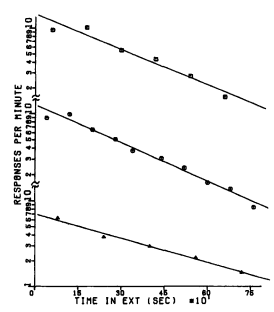
\includegraphics[width = 0.5\textwidth]{graphar}
	\caption{
	Tasas de actividad después de alimento.
	Imagen recuperada de \cite{killeen}}
	\label{fig:grapharousal}


\end{figure}

\clearpage

\section*{Modelo de activación}



El modelo de activación es dado por:

\begin{equation}
R = A\exp^{-t/\alpha}
\end{equation}

	\noindent Donde, $R$ representa la tasa de respuestas esperadas.
	
	\noindent $A$ Es el intercepto de la función cuando $t = 0$, representa la activación del organismo tras el reforzamiento

	\noindent $t$ representa el tiempo transcurrido desde el reforzamiento
	
	\noindent $\alpha$ es la constante de tiempo, que representa el tiempo que debe transcurrir para que la función alcance 0 (indica la tasa de decaimiento de la función)
	
	\noindent Finalmente, la exponencial transforma la función a una escala logarítmica



\bibliographystyle{apacite}
\bibliography{biblioarousal}

\end{document}

